% \begin{figure*}[t]
% \centering
% \begin{subfigure}{0.7\textwidth}
%      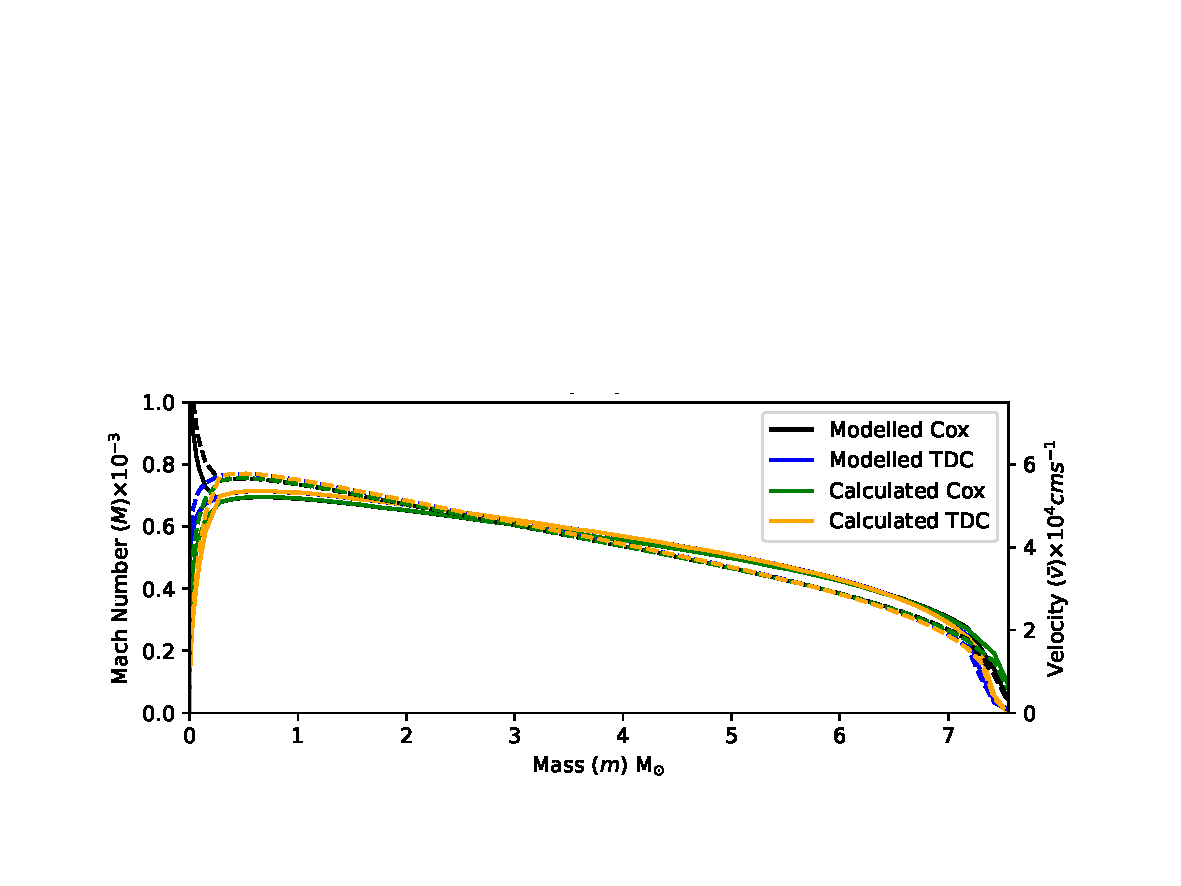
\includegraphics[width=\linewidth]{MachMass_HBurn}
%     \caption{Convection in the core region at $35\%$ core H to burn \\ ($\log \left(\text{time to core collapse}\right)$ is $\sim 6.41\mathrm{yr}$ for both models).}
%     \label{fig:MachMass_HBurn}
% \end{subfigure}

% \hfill
% \begin{subfigure}{\textwidth}
%     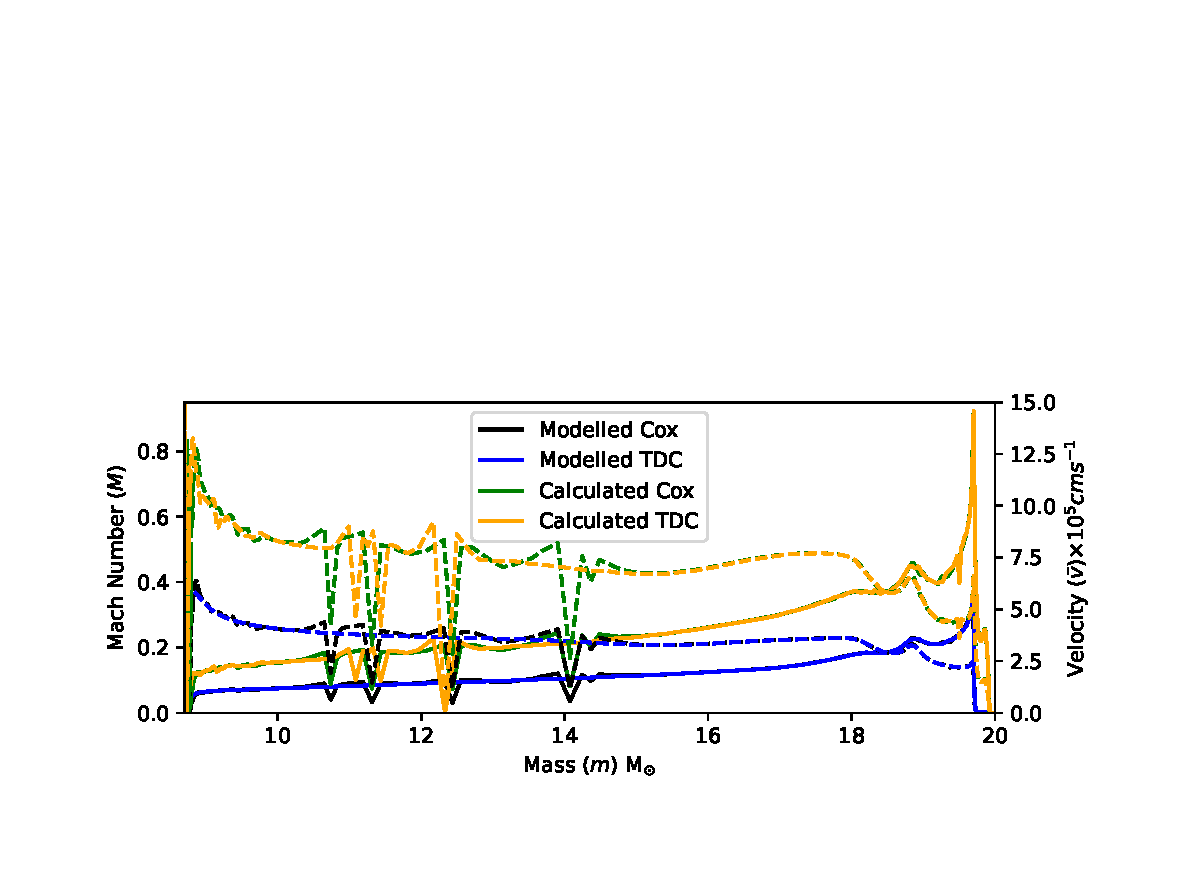
\includegraphics[width=\linewidth]{MachMass_EarlySiBurn}
%     \caption{Convection in the envelope at $95\%$ core Si to burn \\ ($\log \left(\text{time to core collapse}\right)$ is $\sim -2.44\mathrm{yr}$ for \gls{MLT} and $\sim -2.42\mathrm{yr}$ for \gls{TDC}).}
%     \label{fig:MachMass_EarlySiBurn}
% \end{subfigure}
% \hfill
% \begin{subfigure}{0.7\textwidth}
%      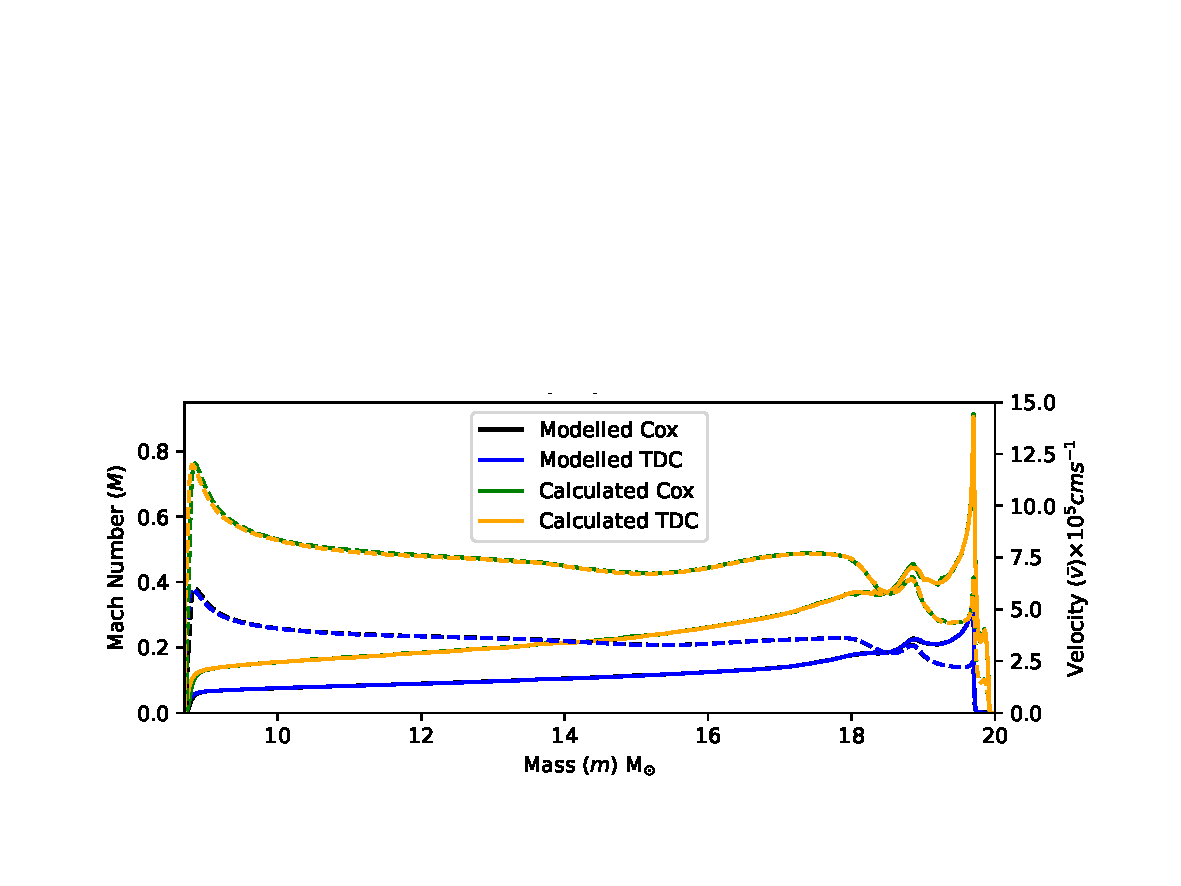
\includegraphics[width=\linewidth]{MachMass_LateSiBurn}
%     \caption{Convection in the envelope at $35\%$ core Si content during O-burning.}
%     \label{fig:MachMass_LateSiBurn}
% \end{subfigure}
% \caption{Graphs of Mach number and convective velocity by mass location. \textit{Modelled} pertains to the use of Equation \ref{eq:ManualVelocityCalc} and \textit{Calculated} to that directly calculated by \texttt{MESA}. Dashed lines are convective velocity measurements and full are of Mach number.}
% \label{fig:MachVel}
% \end{figure*}

% \begin{figure*}[t]   
% \centering
% 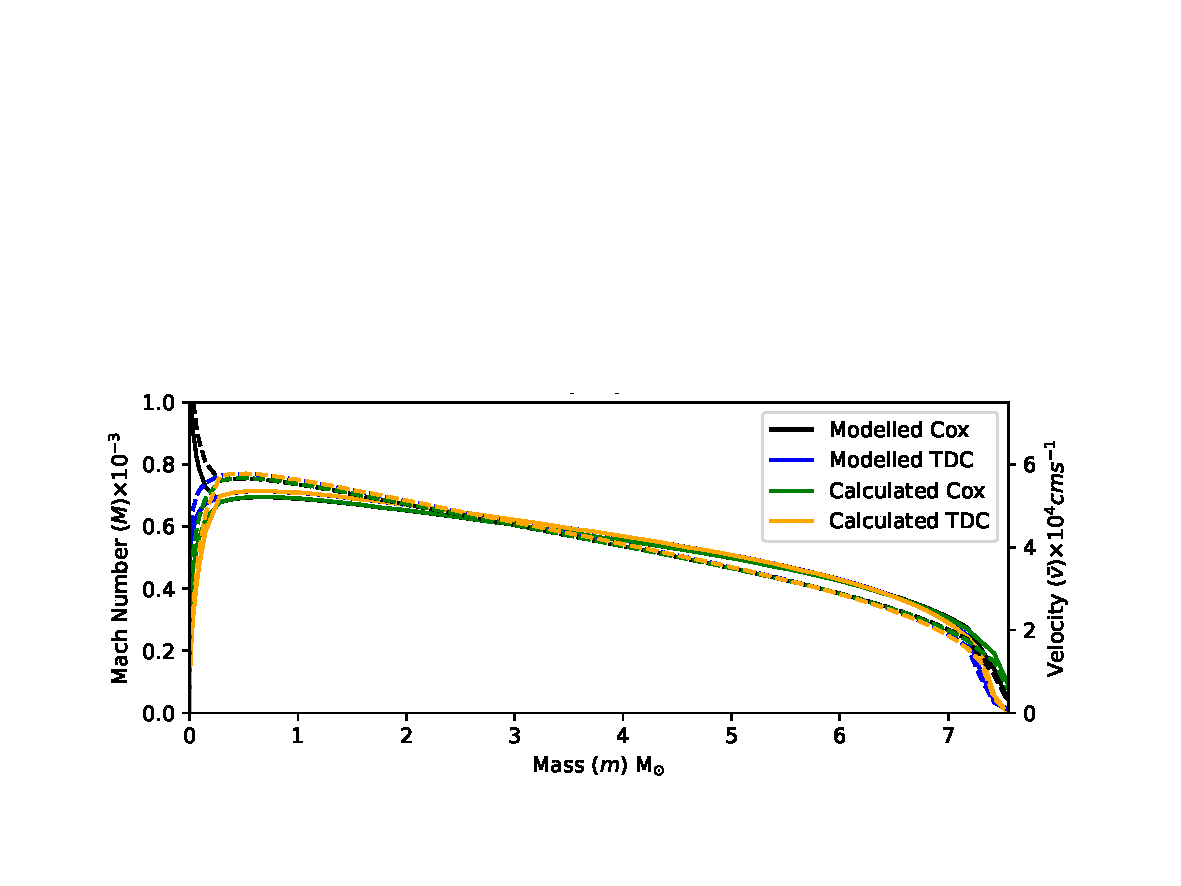
\includegraphics[width=0.8\linewidth]{MachMass_HBurn}
%     \caption{Graph of Mach number and convective velocity by mass location. \textit{Modelled} pertains to the use of Equation \ref{eq:ManualVelocityCalc} and \textit{Calculated} to that directly calculated by \texttt{MESA}. Dashed lines are convective velocity measurements and full are Mach number. Convection shown is in the core region at $35\%$ core H to burn ($\log \left(\text{time to core collapse}\right)$ is $\sim 6.41\mathrm{yr}$ for both models).}
%     \label{fig:MachMass_HBurn}
% \end{figure*}

%%%%%%
\begin{figure*}[t]
\centering
\begin{subfigure}{0.8\textwidth}
     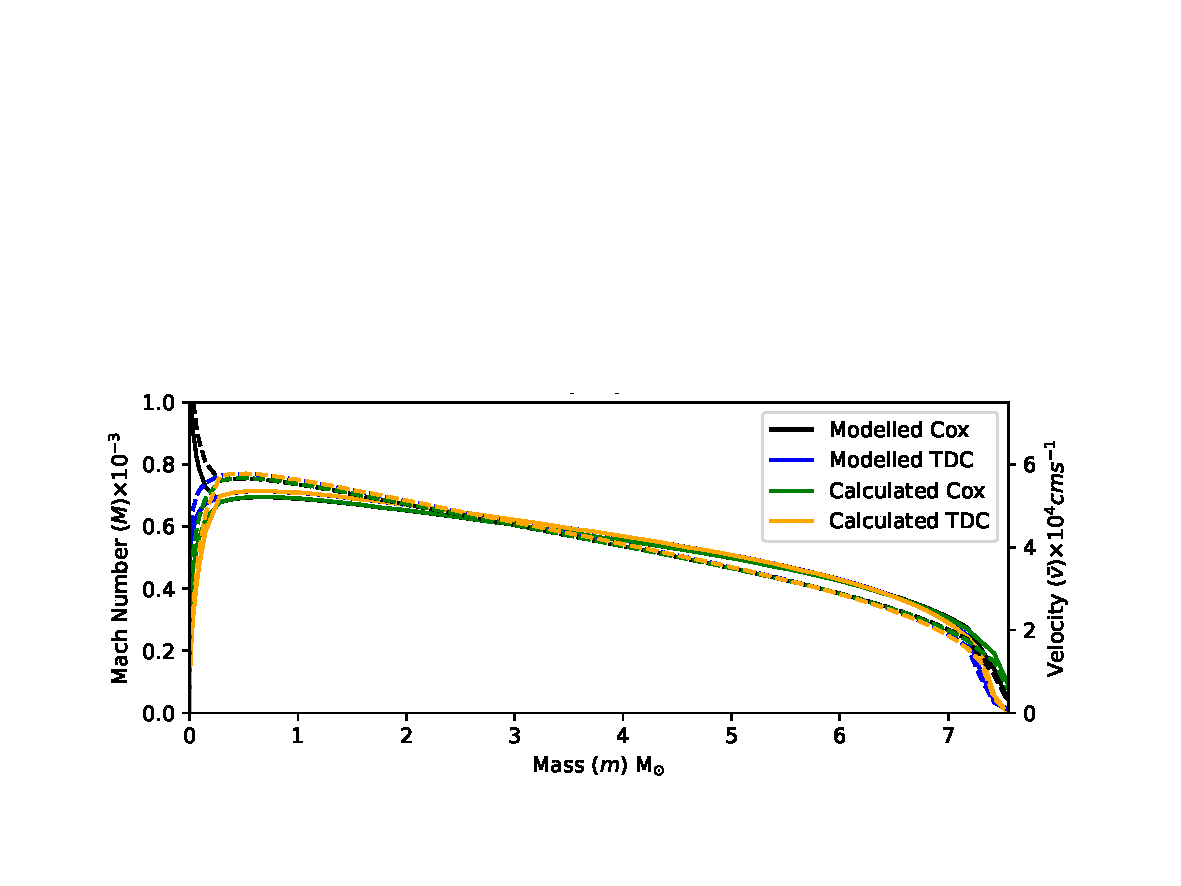
\includegraphics[width=\linewidth]{MachMass_HBurn}
    \caption{Convection shown is in the core region at $35\%$ core H to burn ($\log \left(\text{time to core collapse}\right)$ is $\sim 6.41\mathrm{yr}$ for both models).}
    \label{fig:MachMass_HBurn}
\end{subfigure}
\hfill
\begin{subfigure}{0.8\textwidth}
    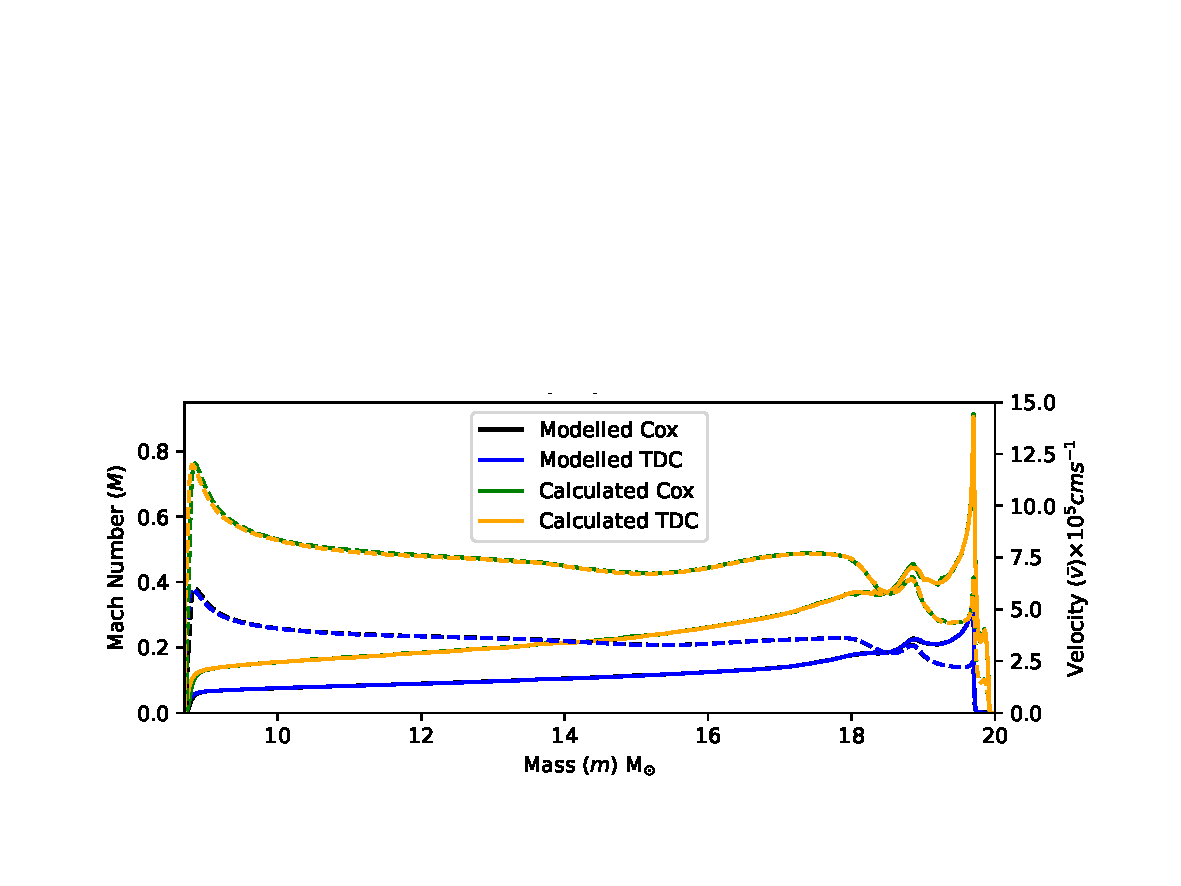
\includegraphics[width=\linewidth]{MachMass_LateSiBurn}
    \caption{Convection in the envelope during O burn, close to core collapse. ($\log \left(\text{time to core collapse}\right)$ is $\sim -0.35\mathrm{yr}$ for \gls{MLT} and $\sim -0.38\mathrm{yr}$ for \gls{TDC}).}
    \label{fig:MachMass_LateSiBurn}
\end{subfigure}
% \hfill
% \begin{subfigure}{0.7\textwidth}
%      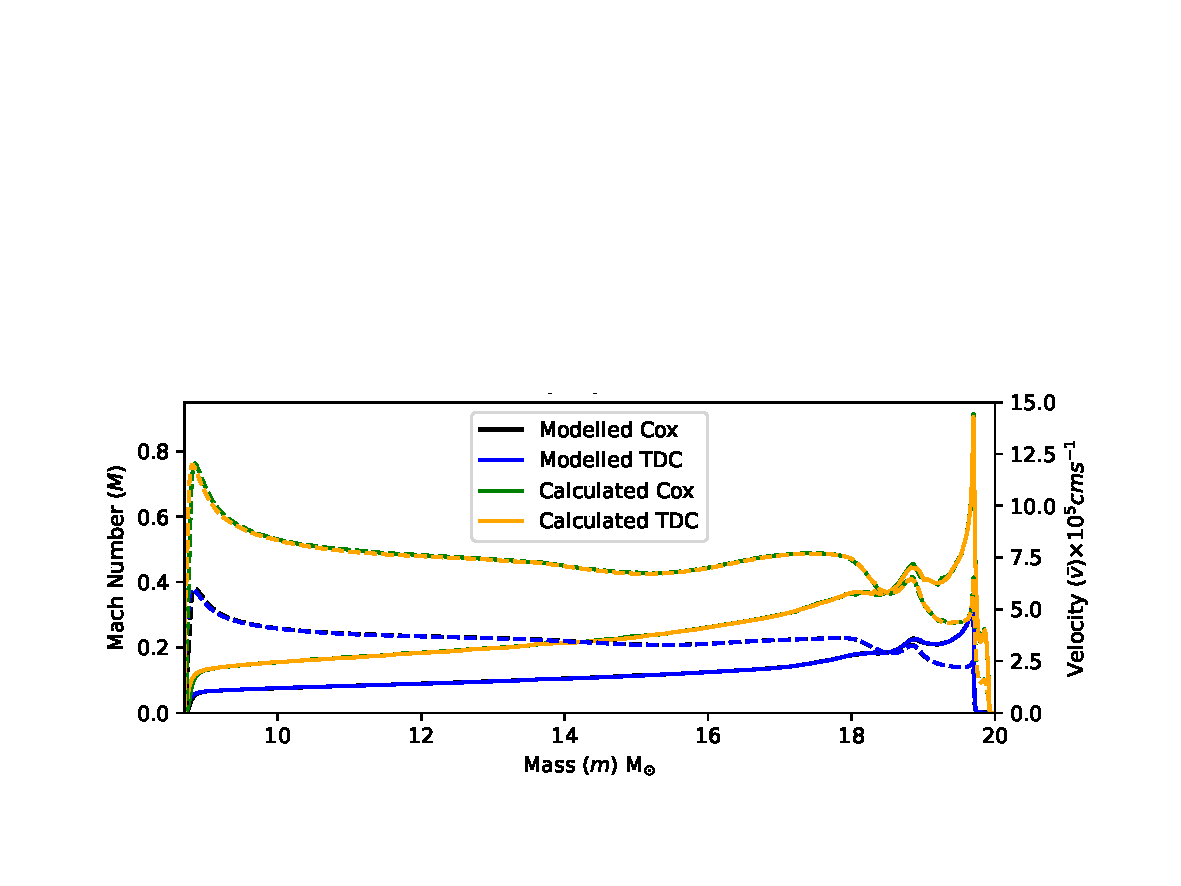
\includegraphics[width=\linewidth]{MachMass_LateSiBurn}
%     \caption{Convection in the envelope at $35\%$ core Si content during O-burning.}
%     \label{fig:MachMass_LateSiBurn}
% \end{subfigure}
\caption{Graphs of Mach number and convective velocity by mass location. \textit{Modelled} pertains to the use of Equation \ref{eq:ManualVelocityCalc} and \textit{Calculated} to that directly calculated by \texttt{MESA}. Dashed lines are convective velocity measurements and full are Mach number.}
\label{fig:MachVel}
\end{figure*}